En los \cref{tab:spherical,tab:linear} se presentan los radios medidos de los
anillos del patrón de interferencia, obtenidos para distintos potenciales de
aceleración en los montajes de tubo esférico y cilíndrico, respectivamente.
Asimismo, se muestra la longitud de onda asociada del electrón \( \lambda \),
calculada a partir de la \cref{eq:wavelength}, junto con su desviación estándar
correspondiente \( \sigma_\lambda \).

\begin{table}[htbp!]
	\centering
	\pgfplotstabletypeset[
	col sep=tab,
	header=true,
	zerofill,
	fixed zerofill,
	fixed,
	columns={0,1,2,3,4},
	columns/0/.style={
		column type={@{}c},
		column name={\text{\(U\) \([\si{\kilo\volt}]\)}},
		fixed zerofill,
		precision=1,
	},
	columns/1/.style={
		column name={\text{\(r_1\) \([\si{\centi\metre}]\)}},
		fixed zerofill,
		precision=3,
	},
	columns/2/.style={
		column name={\text{\(r_2\) \([\si{\centi\metre}]\)}},
		fixed zerofill,
		precision=2,
	},
	columns/3/.style={
		column name={\text{\(\lambda\) \([\si{\pico\metre}]\)}},
		fixed zerofill,
		precision=1,
	},
	columns/4/.style={
		column name={\text{\(\sigma_\lambda\) \([\si{\pico\metre}]\)}},
		column type={c@{}},
	},
	string type,
	every head row/.style={
		before row=\toprule,
		after row=\midrule,
	},
	every cell/.style={math mode},
	every last row/.style={after row=\bottomrule}]{./Data/spherical-data.tsv}
	\vspace{1.5pt}
	\caption{Datos del montaje de Tubo Esférico.}
	\label{tab:spherical-data}
\end{table}


\begin{table}[htbp!]
	\centering
	\pgfplotstabletypeset[
	col sep=tab,
	header=true,
	zerofill,
	columns={0,1,2,3,4},
	columns/0/.style={
		column name={\text{\(U\) \([\si{\kilo\volt}]\)}},
		column type={S[table-format=1.1]},
		fixed zerofill,
		precision=1,
	},
	columns/1/.style={
		column name={\text{\(r_1\) \([\si{\milli\metre}]\)}},
		column type={S[table-format=1.2]},
		fixed zerofill,
		precision=2,
	},
	columns/2/.style={
		column name={\text{\(r_2\) \([\si{\milli\metre}]\)}},
		column type={S[table-format=1.2]},
		fixed zerofill,
		precision=2,
	},
	columns/3/.style={
		column name={\text{\(\lambda\) \([\si{\pico\metre}]\)}},
		column type={S[table-format=1.1]},
		fixed zerofill,
		precision=1,
	},
	columns/4/.style={
		column name={\text{\(\sigma_\lambda\) \([\si{\pico\metre}]\)}},
		column type={S[table-format=1.1]},
	},
	string type,
	every head row/.style={
		before row=\toprule,
		after row=\midrule,
	},
	every last row/.style={after row=\bottomrule}]{./Data/linear-data.tsv}
	\vspace{1.5pt}
	\caption{Datos del montaje de Tubo Plano.}
	\label{tab:linear-data}
\end{table}


Se observa una relación proporcional entre \( r \) y \( \lambda \), en
coincidencia con la teoría.
A partir de una regresión lineal de cada radio en función de la longitud de onda,
se obtienen las \cref{fig:regression-spherical,fig:regression-cylinder}.
Utilizando las pendientes obtenidas y las relaciones \cref{eq:parameter-spherical,eq:parameter-linear},
se determinan los parámetros de distancia interplanar presentados en \cref{tab:parameters}.

\begin{figure}[htbp!]
  \centering
  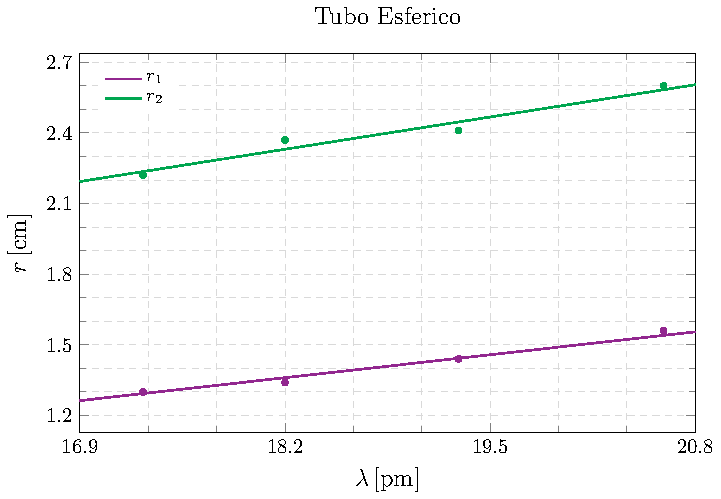
\includegraphics[width=\linewidth]{./Figures/spherical-graph.pdf}
  \caption{Regresión lineal de los datos obtenidos con el montaje de tubo esférico.}
  \label{fig:regression-spherical}
\end{figure}

\begin{figure}[htbp!]
  \centering
  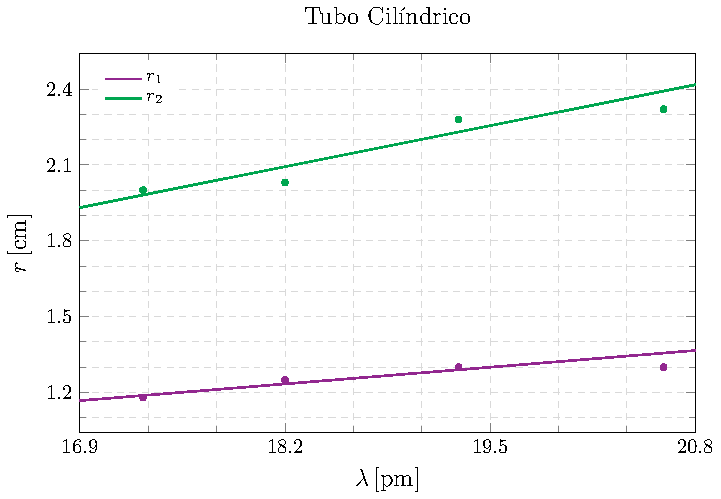
\includegraphics[width=\linewidth]{./Figures/linear-graph.pdf}
  \caption{Regresión lineal de los datos obtenidos con el montaje de tubo cilíndrico.}
  \label{fig:regression-cylinder}
\end{figure}

\begin{table}[htbp!]
  \centering
  \begin{tabular}{@{}ccS[table-format=3.1]@{}}
    \toprule
    Tubo & \(r\) & {\(d\) \([\si{\pico\metre}]\)} \\
    \midrule
    \multirow{2}{*}{Esférico} & \(r_1\) & 173.5 \\
                              & \(r_2\) & 123.4 \\
    \midrule
    \multirow{2}{*}{Cilíndrico} & \(r_1\) & 265.6 \\
                                 & \(r_2\) & 108.4 \\
    \bottomrule
  \end{tabular}
  \vspace{1.5pt}
  \caption{Parámetros de distancia interplanar obtenidos.}
  \label{tab:parameters}
\end{table}


Los radios interiores se originan debido a una mayor distancia recorrida por
los electrones, lo que se refleja en los valores obtenidos para \( d \).
